\section{Monitoring and Analytics}
\label{sec:monitoring-analytics}

The FLOPY-NET framework incorporates comprehensive monitoring and analytics capabilities to provide real-time insights into federated learning operations, network performance, and system health. This section details the monitoring infrastructure, analytics pipeline, and visualization capabilities.

\subsection{Monitoring Architecture}

The monitoring system follows a multi-layer architecture that captures metrics at different levels of the system:

\begin{figure}[htbp]
\centering
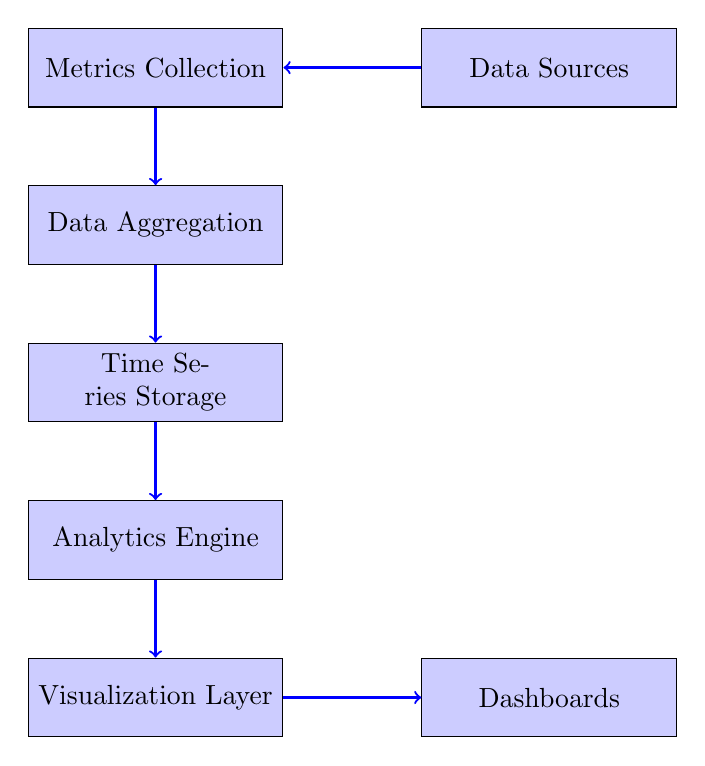
\begin{tikzpicture}[
    node distance=2cm,
    box/.style={rectangle, draw, fill=blue!20, text width=3cm, text centered, minimum height=1cm},
    arrow/.style={->, thick, blue}
]
    % Monitoring Layers
    \node[box] (metrics) {Metrics Collection};
    \node[box, below of=metrics] (aggregation) {Data Aggregation};
    \node[box, below of=aggregation] (storage) {Time Series Storage};
    \node[box, below of=storage] (analytics) {Analytics Engine};
    \node[box, below of=analytics] (visualization) {Visualization Layer};
    
    % Connections
    \draw[arrow] (metrics) -- (aggregation);
    \draw[arrow] (aggregation) -- (storage);
    \draw[arrow] (storage) -- (analytics);
    \draw[arrow] (analytics) -- (visualization);
    
    % Side components
    \node[box, right of=metrics, xshift=3cm] (sources) {Data Sources};
    \node[box, right of=visualization, xshift=3cm] (dashboards) {Dashboards};
    
    \draw[arrow] (sources) -- (metrics);
    \draw[arrow] (visualization) -- (dashboards);
\end{tikzpicture}
\caption{Monitoring Architecture Overview}
\label{fig:monitoring-arch}
\end{figure}

\subsection{Metrics Collection}

The system collects various types of metrics across different components:

\subsubsection{System Metrics}
\begin{itemize}
    \item \textbf{Resource Utilization}: CPU, memory, disk, and network usage
    \item \textbf{Container Metrics}: Docker container performance and health
    \item \textbf{Network Metrics}: Bandwidth utilization, latency, packet loss
    \item \textbf{Application Metrics}: Request rates, response times, error rates
\end{itemize}

\subsubsection{Federated Learning Metrics}
\begin{itemize}
    \item \textbf{Training Metrics}: Model accuracy, loss functions, convergence rates
    \item \textbf{Communication Metrics}: Model update sizes, transmission times
    \item \textbf{Participation Metrics}: Client availability, dropout rates
    \item \textbf{Security Metrics}: Authentication attempts, encryption overhead
\end{itemize}

\subsection{Data Collection Implementation}

The monitoring system uses multiple collection agents and exporters:

\begin{lstlisting}[language=yaml, caption=Prometheus Configuration]
global:
  scrape_interval: 15s
  evaluation_interval: 15s

scrape_configs:
  - job_name: 'flopy-net-services'
    static_configs:
      - targets: ['policy-engine:8080', 'dashboard:3000', 'collector:5000']
    metrics_path: /metrics
    scrape_interval: 10s
    
  - job_name: 'node-exporter'
    static_configs:
      - targets: ['node-exporter:9100']
      
  - job_name: 'cadvisor'
    static_configs:
      - targets: ['cadvisor:8080']
\end{lstlisting}

\subsection{Analytics Pipeline}

The analytics pipeline processes collected metrics to generate insights:

\begin{figure}[htbp]
\centering
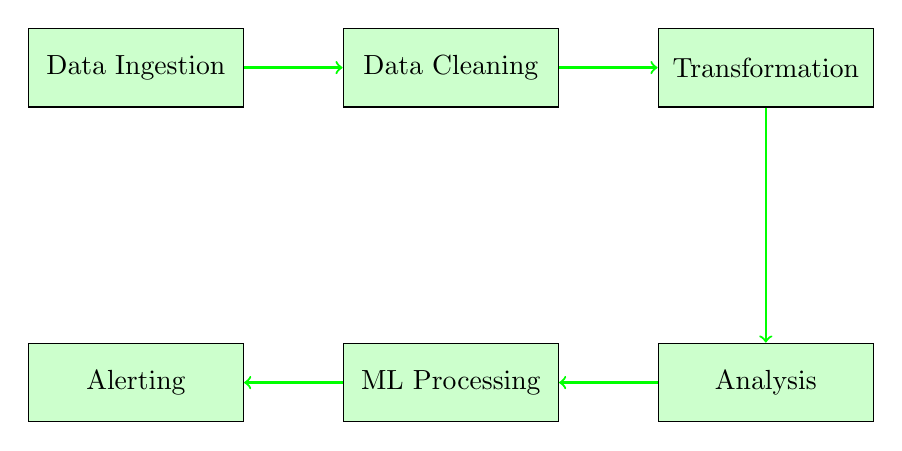
\begin{tikzpicture}[
    node distance=4cm,
    process/.style={rectangle, draw, fill=green!20, text width=2.5cm, text centered, minimum height=1cm},
    arrow/.style={->, thick, green}
]
    \node[process] (ingest) {Data Ingestion};
    \node[process, right of=ingest] (clean) {Data Cleaning};
    \node[process, right of=clean] (transform) {Transformation};
    \node[process, below of=transform] (analyze) {Analysis};
    \node[process, left of=analyze] (ml) {ML Processing};
    \node[process, left of=ml] (alert) {Alerting};
    
    \draw[arrow] (ingest) -- (clean);
    \draw[arrow] (clean) -- (transform);
    \draw[arrow] (transform) -- (analyze);
    \draw[arrow] (analyze) -- (ml);
    \draw[arrow] (ml) -- (alert);
\end{tikzpicture}
\caption{Analytics Pipeline Flow}
\label{fig:analytics-pipeline}
\end{figure}

\subsection{Real-time Analytics}

The system provides real-time analytics capabilities for immediate insights:

\subsubsection{Stream Processing}
\begin{lstlisting}[language=python, caption=Stream Processing Implementation]
import asyncio
import json
from kafka import KafkaConsumer
from prometheus_client import Gauge, Counter

class MetricsProcessor:
    def __init__(self):
        self.consumer = KafkaConsumer(
            'metrics-topic',
            bootstrap_servers=['kafka:9092'],
            value_deserializer=lambda x: json.loads(x.decode('utf-8'))
        )
        
    async def process_metrics(self):
        for message in self.consumer:
            metric_data = message.value
            await self.analyze_metric(metric_data)
            
    async def analyze_metric(self, data):
        # Real-time metric analysis
        if data['type'] == 'fl_accuracy':
            self.update_accuracy_gauge(data['value'])
        elif data['type'] == 'system_resource':
            self.check_resource_thresholds(data)
\end{lstlisting}

\subsection{Visualization Dashboard}

The monitoring system includes comprehensive dashboards for different stakeholders:

\subsubsection{Operational Dashboard}
\begin{itemize}
    \item System health overview
    \item Resource utilization trends
    \item Service availability status
    \item Alert notifications
\end{itemize}

\subsubsection{Federated Learning Dashboard}
\begin{itemize}
    \item Training progress visualization
    \item Model performance metrics
    \item Client participation statistics
    \item Communication efficiency metrics
\end{itemize}

\subsubsection{Network Performance Dashboard}
\begin{itemize}
    \item Network topology visualization
    \item Bandwidth utilization
    \item Latency heatmaps
    \item Quality of Service metrics
\end{itemize}

\subsection{Alerting System}

The monitoring system includes intelligent alerting capabilities:

\begin{lstlisting}[language=yaml, caption=Alert Rules Configuration]
groups:
  - name: flopy-net-alerts
    rules:
      - alert: HighCPUUsage
        expr: cpu_usage_percent > 80
        for: 5m
        labels:
          severity: warning
        annotations:
          summary: "High CPU usage detected"
          
      - alert: ModelAccuracyDrop
        expr: fl_model_accuracy < 0.7
        for: 2m
        labels:
          severity: critical
        annotations:
          summary: "Model accuracy dropped below threshold"
          
      - alert: ClientDropout
        expr: fl_active_clients < fl_required_clients * 0.8
        for: 1m
        labels:
          severity: warning
        annotations:
          summary: "High client dropout rate detected"
\end{lstlisting}

\subsection{Log Management}

Comprehensive log management ensures system observability:

\subsubsection{Centralized Logging}
\begin{itemize}
    \item ELK Stack (Elasticsearch, Logstash, Kibana) integration
    \item Structured logging with JSON format
    \item Log correlation across distributed components
    \item Automated log retention policies
\end{itemize}

\subsubsection{Log Analytics}
\begin{itemize}
    \item Error pattern detection
    \item Performance bottleneck identification
    \item Security event correlation
    \item Compliance audit trails
\end{itemize}

\subsection{Performance Optimization}

The monitoring system enables continuous performance optimization:

\subsubsection{Automated Optimization}
\begin{lstlisting}[language=python, caption=Auto-scaling Implementation]
class AutoScaler:
    def __init__(self, metrics_client):
        self.metrics = metrics_client
        self.thresholds = {
            'cpu_high': 80,
            'memory_high': 85,
            'response_time_high': 2.0
        }
        
    async def monitor_and_scale(self):
        while True:
            metrics = await self.metrics.get_current_metrics()
            
            if self.should_scale_up(metrics):
                await self.scale_up_services()
            elif self.should_scale_down(metrics):
                await self.scale_down_services()
                
            await asyncio.sleep(30)  # Check every 30 seconds
\end{lstlisting}

\subsection{Compliance and Auditing}

The monitoring system supports compliance and auditing requirements:

\begin{itemize}
    \item \textbf{Data Governance}: Tracking data lineage and usage
    \item \textbf{Privacy Compliance}: Monitoring data access and processing
    \item \textbf{Security Auditing}: Logging security events and access patterns
    \item \textbf{Regulatory Reporting}: Automated compliance report generation
\end{itemize}

\subsection{Integration with External Systems}

The monitoring system integrates with external tools and platforms:

\begin{itemize}
    \item \textbf{SIEM Integration}: Security Information and Event Management
    \item \textbf{ITSM Integration}: IT Service Management platforms
    \item \textbf{Cloud Monitoring}: Integration with cloud provider monitoring services
    \item \textbf{Third-party Analytics}: Integration with specialized analytics platforms
\end{itemize}

This comprehensive monitoring and analytics infrastructure ensures that the FLOPY-NET system operates efficiently, securely, and reliably while providing stakeholders with the insights needed for informed decision-making.
